\section{Progettazione}

\subsection{Embodiment}

Per la realizzazione del modello del robot ci si è basati su quella di \href{https://www.cyberbotics.com/e-puck}{E-puck v2}, a cui vi sono stati aggiunti una serie di sensori extra (\textit{Bumpers}) al fine di mantenere il modello coerente a quello descritto in \cite{pfeifer2001understanding} e che fosse un buon compromesso rispetto a quello descritto in \cite{verschure1992distributed}.

\subsubsection{Sensori}

Ci limiteremo a descrivere i sensori utilizzati nella nostra versione di E-puck e utili ai fini dell'esperimento. Per la precisione verranno specificate le caratteristiche in termini di range, rumore e mapping definiti tramite le Look-Up Table che governano il comportamento di tali sensori.

\begin{itemize}
    \item \texttt{IR Distance Sensor}: Tali sensori sono queli di default presenti in E-puck. Nel nostro caso specifico sono stati programmati per ottenere una risoluzione minima di \texttt{0cm} e massima di \texttt{10cm}, con un rumore variabile tra \texttt{[0.01, 0.05]}. Per restare allineati con i valori sia del paper \cite{verschure1992distributed} che del libro \cite{pfeifer2001understanding}, si è deciso di mappare i valori simulati percepiti dal sensore in un intorno compreso tra \texttt{[0.0, 1.0]}.
    
    \item \texttt{Bumper Sensor}: Tali sensori sono stati aggiunti al modello base di E-puck al fine di modellare lo Stimolo non-Condizionato (US \cite{verschure1992distributed}) che porta l'agente a modificare la velocità delle proprie ruote e dunque spostarsi dall'ostacolo (UR \cite{verschure1992distributed}).
    Come per il sensore precedente, per restare allineati ai documenti di riferimento, la Look-Up Table è stata così definita: il sensore produce valori \texttt{\{0.0, 1.0\}} a seconda che sia avvenuta o meno una collisione, con un rumore pari a \texttt{0.01}\footnote{Ma non dovrebbe fare molta differenza porlo anche a 0.0 visto che il sensore è binario.}. I valori del sensore sono poi mappati in maniera identica in \texttt{\{0, 1\}}.
\end{itemize}

\newpage

\subsubsection{Effettori}

Gli unici effettori di cui è provvisto il nostro modello di E-puck sono i \texttt{Rotational Motor} che permettono di modulare la potenza e direzione della rotazione di una singola ruota. Dal momento che l'agente è provvisto di 2 sole ruote (una per ogni lato), sono anche presenti 2 \texttt{Rotational Motor}. Tali motori producono una velocità lineare per ogni ruota compresa tra \texttt{[0.0, 7.536]cm/sec}.

\subsubsection{Morfologia}

\begin{figure}[H]
    \centering
    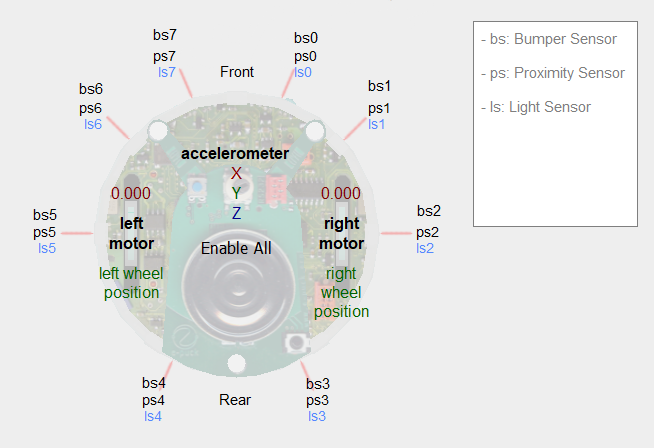
\includegraphics[scale=0.9]{figures/epuck_morphology.png}
    \caption{La morfologia del robot è quella classica del modello E-puck. I bumpers sono stati posizionati in corrispondenza di ogni \texttt{Distance Sensor} (in figura \texttt{ps}), ma in modo tale da non ostruire il raggio d'azione del sensore. Nello specifico sono posizionati attorno alla circonferenza del cilindro che costituisce il corpo principale alle senguenti angolature (leggendo in senso orario, da \texttt{bs0} a \texttt{bs7}): \texttt{1.27rad}, \texttt{0.77rad}, \texttt{0.0rad}, \texttt{5.21rad}, \texttt{4.21rad}, \texttt{3.14159rad}, \texttt{2.37rad}, \texttt{1.87rad}.}
    \label{fig:Morphology}
\end{figure}

\newpage

\subsection{Neural Network Controller}\label{lab:ANN}

Dal momento che le descrizioni dell'esperimento nei documenti di riferimento \cite{pfeifer2001understanding, verschure1992distributed} non sono totalmente coerenti dal punto di vista della descrizione del controller e della morfologia del robot utilizzato, si è deciso di realizzare più versioni del controller (\textit{senza modificarne la morfologia}). Ogni versione sfrutta o aggrega solo una parte dei sensori equipaggiati.

\paragraph{Differenze nei modelli di riferimento}
All'interno di \cite{pfeifer2001understanding} viene modellato un robot che possiede 6 sensori di prossimità affiancati ognuno da un sensore di collisione. Tali sensori sono montati lungo la metà anteriore del robot. I sensori di prossimità sono collegati ad un primo layer di 6 neuroni, i quali utilizzano una Sigmoide come funzione di attivazione. Tale layer di neuroni è a sua volta \textit{Fully Connected} con pesi variabili ad un secondo layer di input composto da ulteriori 6 neuroni. Ognuno di questi ultimi riceve in input anche il segnale proveniente da uno dei sensori di collisione. Nel secondo layer la funzione di attivazione utilizzata è la \textit{Binary Threshold}. L'incognita del modello esposto dal libro sono le connessioni del Layer di Collisione con i neuroni del layer successivo, il Motor Layer, che ne implementa i riflessi: ogni neurone del Layer di Collisione è collegato a gruppi di due ai 3 neuroni del Motor Layer. I riflessi inoltre non sono delineati all'interno della descrizione fornita e non è specificato quali azioni applicano sui motori. 


All'interno di \cite{verschure1992distributed} è presentato un controller che implementa \textit{Obstacle-Avoidance} e \textit{Fototassi}. Proseguiamo la spiegazione concentrandoci solo sulla componente di \textit{Obstacle-Avoidance}. 
Il modello proposto dal paper è provvisto di 6 sensori di prossimità, posizionati nella parte anteriore dell'agente tra $[90\degree,-90\degree]$, e 2 sensori di collisione che rivestono i due quarti anteriori del veicolo tra $[90\degree,-90\degree]$. Non è specificato il numero di ruote di cui è provvisto il robot.
In tale documento, inoltre, non si fa specificatamente riferimento all'uso di una rete neurale, bensì si parla genericamente di "\textit{learning mechanisms}" e "\textit{neural fields}", richiamandosi per la maggior parte al \textit{Classical Conditioning} e i \textit{Value System}. Nel paper l'apprendimento è infatti identificato come l'associazione di una serie di \textit{stimuli} ad una specifica \textit{response}. 

Nello specifico vengono delineati:

\begin{itemize}
    \item \textit{Conditioned-Stimuli}, associabili ai segnali percepiti dall'agente tramite i sensori di prossimità. Tali \textit{stimuli} sono organizzati in \textit{Conditioned-Stimuli Fields}. Questo "layer" modula il segnale degli \textit{stimuli} utilizzando una funzione esponenziale inversa come una funzione di attivazione.
    
    \item \textit{Unconditioned-Stimuli$^-$}, associabili ai segnali percepiti dall'agente tramite i sensori di collisione. In questo caso gli \textit{stimuli} sono organizzate in \textit{Unconditioned-Stimuli Fields$^-$}. Tali \textit{stimuli} sono collegati agli elementi dei \textit{Conditioned-Stimuli Fields} da una serie di connessioni (variabili) che vanno da quest'ultimo verso il primo.
    
    \item \textit{Unconditioned-Response}, associabili ai segnali da inviare ai motori al fine di ottenere un certo comportamento. Tali \textit{response} sono organizzati in \textit{Unconditioned-Response Fields} e ad ognuna è associato ad un "\textit{command neuron}" che ne codifica la precisa risposta ai motori (un riflesso). Tali \textit{response} sono delineate nel paper come \texttt{Advance}, \texttt{Reverse}, \texttt{TurnLeft(x degrees)} e \texttt{TurnRight(x degrees)} ma senza approfondire ne la loro implementazione, ne la loro interazione o eventuale mutua esclusione.
    
    Ogni \textit{command neuron} è collegato agli elementi dei \textit{Unconditioned-Stimuli Fields$^-$} tramite una serie di connessioni pesate e fisse che vanno da quest'ultimo verso il primo.
\end{itemize}  

Di conseguenza abbiamo deciso di semplificare il modello ponendo solo 2 neuroni nel Motor Layer che singolarmente pilotano ciascuno la propria ruota e un solo neurone nel Reverse Layer che agisce sull'output dei neuroni del motor layer modificandone il segno.
Il comportamento della sterzata risulterà emergente dalle differenti velocità "erogate" ai due motori.
Questa idea è nata seguendo l'esempio dei \textit{Braitenberg Vehicles}.

Questo tipo di modellazione inoltre riduce il problema della \textit{Behaviour Segmentation} ed una gestione altrimenti macchinosa dell'interazione tra i riflessi.

\subsubsection{Struttura generale}

\begin{figure}[H]
    \centering
    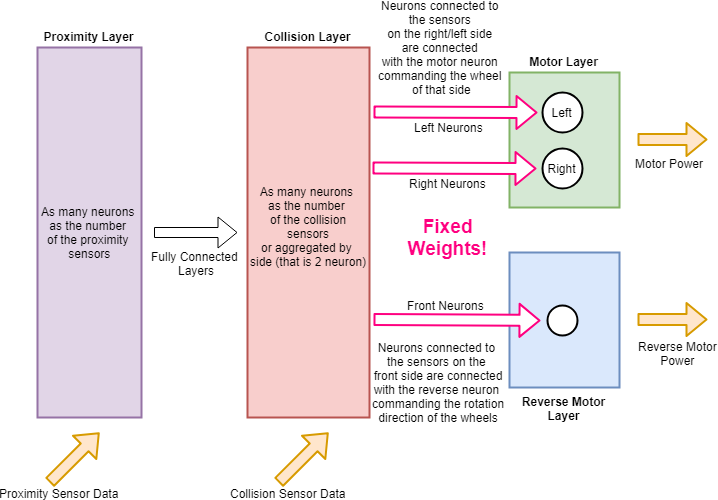
\includegraphics[scale=0.6]{figures/dac_ann_structure_generic.png}
    \caption{In figura è presentata la struttura della rete neurale, ad alto livello e generalizzata, adoperata per implementare il controller.\\ 
    Il numero dei neuroni nei layer di input dipenderà dalla configurazione dei sensori o dalle possibili astrazioni applicate su di essi. L'apprendimento inoltre avviene solo sulle connessioni presenti tra il layer di prossimità e quello di collisione.\\ 
    Tutte le altre connessioni sono fisse e poste a \texttt{1.0}. 
    Il numero di neuroni nel layer di output, invece, dipende dal numero di riflessi che si vogliono implementare nel robot. 
    Nel nostro caso l'agente deve solo eseguire l'\texttt{Obstacle-Avoidance}, di conseguenza si è posto un solo neurone per ruota che ne pilota la potenza del motore associato e un solo neurone che inverte il senso di rotazione di una di esse, necessario se il robot vuole evitare scontri frontali (inversione di marcia), per un totale quindi di 3 neuroni.}
    \label{fig:AnnStructure}
\end{figure}

\newpage

Partendo quindi dalle due strutture di riferimento sono quindi state realizzate 3 versioni del controller, tutte caratterizzate da una configurazione neurale peculiare.\label{marker:dacmodels} 
\begin{enumerate}
    \item La prima versione, visibile in figura \ref{fig:dacv2} e denominata \texttt{dacv2}, sfrutta tutti i sensori di prossimità e bumper presenti. Gli output dei sensori di prossimità sono collegati come input ai neuroni del \textit{proximity layer}. Quest'ultimi sono poi fully connected con pesi variabili ai neuroni del \textit{collision layer}, in cui ad ogni neurone di tale livello è associato un bumper. Successivamente i neuroni collegati ai bumper del lato sinistro dell'agente sono collegati ad un neurone che mappa gli input nella relativa risposta al motore che pilota la ruota sinistra. Rispettivamente i neuroni di collisione relativi al lato destro sono collegati ad un neurone che modella la risposta al motore del lato destro. Per quanto riguarda i neuroni a cui sono collegati i bumper frontali (\textit{bs0 e bs7}), essi sono anche collegati ad un neurone dedito all'attivazione del riflesso di inversione del motore. Tutti i collegamenti dal layer di collisione a quello della gestione delle risposte dei motori presentano pesi fissi.
    
    \item Nella successiva versione, denominata \texttt{dacv3} si è cercato di fornire un'implementazione simile a quella riportata nel paper \cite{verschure1992distributed}.
    In esso si ha che il robot possiede solamente 2 sensori di collisione frontali, i quali coprono rispettivamente metà della parte anteriore del robot (1/4 della circonferenza del robot). All'interno del simulatore utilizzato non vi è la possibilità di utilizzare bumper di tali dimensioni, per cui si è pensato di utilizzare gli stessi bumper della versione \textit{dacv2} e modellare i bumper descritti nel paper sfruttando la somma logica dei segnali provenienti dai bumper che coprono la relativa posizione di quelli del paper. Tale somma logica verrà poi utilizzata all'interno della funzione di composizione dei neuroni del livello di collisione.
    Come descritto in figura \ref{fig:Dacv3} si avrà quindi che per quanto riguarda la gestione del layer di prossimità è stata utilizzata la stessa configurazione della versione \textit{dacv2}. Questo layer è fully connected a 3 neuroni nel livello di collisione ai quali sono collegati rispettivamente i bumper [\textit{bs0,bs1,bs2}] (la cui somma logica modella il bumper del paper montato sulla parte destra), [\textit{bs3 e bs4}] e [\textit{bs5,bs6,bs7}] (la cui somma logica modella il bumper del papar montato a sinistra). Successivamente il neurone che si occupa di rilevare le collissioni a destra è collegato al neurone che mappa la risposta del motore destro e viceversa per quanto riguarda i neuroni del livello di collisione e dei motori della parte sinistra. Entrambe le uscite dei neuroni di destra e sinistra del livello di collisione sono collegate al neurone che gestisce il riflesso di reverse. Per quanto riguarda il neurone del livello di collisione centrale (\ref{fig:Dacv3}) quello che riceve gli input dai bumpers \textit{bs3 e bs4} esso al momento non è collegato a nessun neurone del layer motori. Esso è stato comunque lasciato in quanto in futuro potrebbe essere utilizzato per implementare la gestione del riflesso "advance" citato nel paper, che al fine della collision-avoidance non è risultato necessario.
    
    \item Partendo dall'implementazione della versione \textit{dacv2} si è realizzata un'ultima versione, denominata \texttt{dacv4}(visibile in figura \ref{fig:dacv4}),  in cui i sensori di prossimità posteriori \texttt{\{ps3, ps4\}} e i relativi bumpers \texttt{\{bs3, bs4\}} sono scollegati dal controller. Ergo, vengono adoperati ai fini dell'apprendimento esclusivamente i sensori di prossimità e bumper frontali e laterali. Tale implementazione è nata dalla necessità di capire se l'uso dei sensori posteriori influisse negativamente sull'apprendimento generale del robot.
    
\end{enumerate}

\begin{figure}[H]
    \centering
    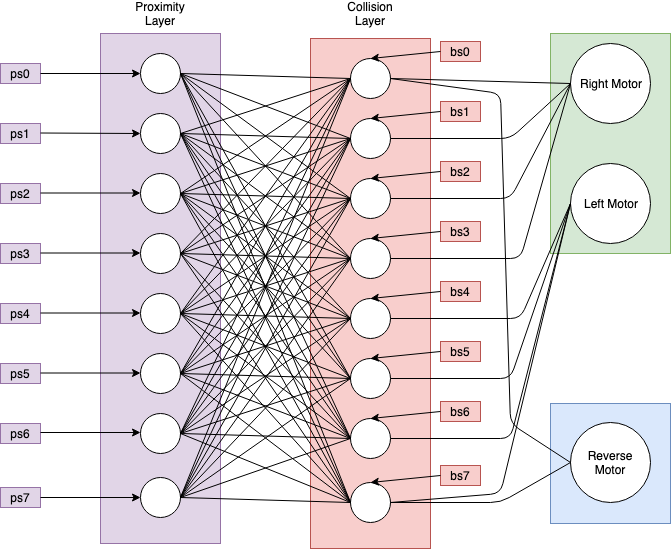
\includegraphics[scale=0.45]{figures/NetVersion2.png}
    \caption{Schema della rete \texttt{dacv2}}
    \label{fig:dacv2}
\end{figure}

\begin{figure}[H]
    \centering
    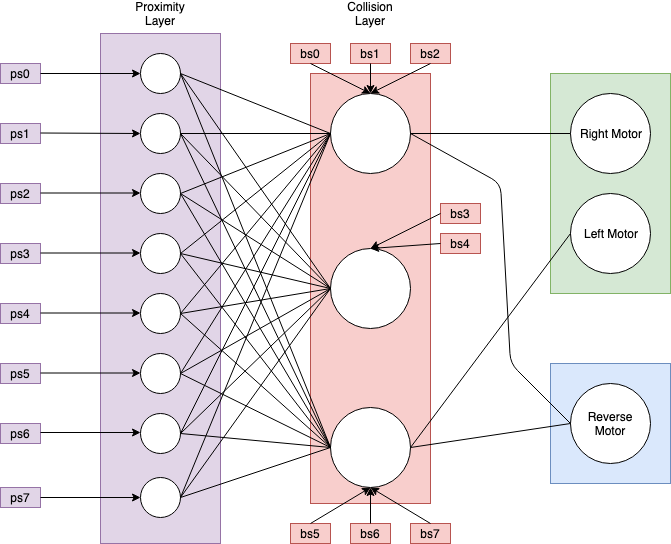
\includegraphics[scale=0.45]{figures/NetVersion3.png}
    \caption{Schema della rete \texttt{dacv3}}
    \label{fig:Dacv3}
\end{figure}

\begin{figure}[H]
    \centering
    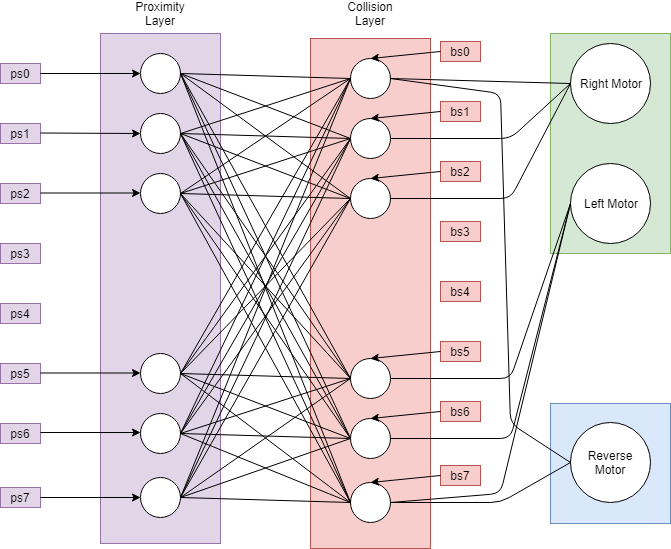
\includegraphics[scale=0.45]{figures/NetVersion4.png}
    \caption{Schema della rete \texttt{dacv4}}
    \label{fig:dacv4}
\end{figure}

In tutte e tre le versioni il layer di "reverse" contiene un solo neurone che si deve attivare qualora tutti i neuroni del layer di collisione associati con i bumper frontali risultano attivi. Il verso della marcia dipenderà dall'eventuale numero degli altri neuroni attivi nel layer di collisione e a quale lato (sinistro o destro) questi fanno parte. Il lato che possiede meno neuroni attivi assume marcia negativa. In caso di parità sarà sempre il motore di destra ad assumere senso negativo.

% \newpage

\subsubsection{Input Composition, Activation  Functions e Output Functions}

Prima di esporre le varie formule vogliamo fare dei chiarimenti sulla notazione usata, nello specifico negli indici, al fine di evitare confusione e velocizzare la compresione di ciò che viene riportato.

\begin{itemize}
    \item Indice ${i}$ indica sempre una entità del Layer precedente
    \item Indice ${k}$ indica sempre una entità proveniente dai sensori, usualmente $k==j$
    \item Indice ${j}$ indica sempre una entità del layer attuale
    \item $w_{ij}$ è il peso della connessione tra il neurone $i$ del livello precedente ed il neurone $j$ del layer successivo
    \item $N_j$ è l'insieme di neuroni del layer precedente connessi al neurone $j$ del layer successivo
    \item $o_j$ è l'output del neurone $j$ del layer corrente
    \item $o_i$ è l'output del neurone $i \in N_j$ appartenente al layer precedente
\end{itemize}

\newpage

\textbf{Proximity} = $
    \begin{cases}
        h_j=p_k & \text{where $p_k$ is the output of sensor $ps_k$} \\
        a_j=e^{-h_j} & \\
        o_j=a_j & \\
    \end{cases}
$\\

\hfill\break

\textbf{Collision} = $
    \begin{cases}
        h_j = c_k + \sum_{i\in N_j} w_{ij}\cdot o_i \\
        a_j = \begin{cases}
           1 & \text{if $h_j \ge \tau_{Collision}$,}\\
           0 & \text{else.}
        \end{cases} & \\
        o_j = a_j & \\
    \end{cases}
$\\

\hfill\break
Where $c_k$ is the output of sensor $bs_k$ in net versions \textit{dacv2 and dacv4} and is the logic sum of outputs of $bs$ sensors connected to the neuron in net version \textit{dacv3}. 

\hfill\break

\textbf{Reverse} = $
    \begin{cases}
        h_j = \sum_{i\in N_j} w_{ij}\cdot o_i & \\
        a_j = \begin{cases}
           1 & \text{if $h_j \ge \tau_{Reverse}$,}\\
           0 & \text{else.}
        \end{cases} & \\
        o_j = a_j & \\
    \end{cases}
$\\

\hfill\break

\textbf{Motor} = $
    \begin{cases}
        h_j = \sum_{i\in N_j} w_{ij}\cdot o_i & \\
        a_j = \begin{cases}
           h_j & \text{if $h_j \ge \tau_{Motor}$,}\\
           0 & \text{else.}
        \end{cases} & \\
        o_j = a_j \cdot \texttt{MIN\_V} & \text{where \texttt{MIN\_V} is a bounding constant} \\
    \end{cases}
$\\

\hfill\break

La funzione di attivazione nel Motor Layer potrebbe tranquillamente essere una funzione linerare tale che $a_j=h_j$. Il comportamento risultante è il medesimo.

\newpage

\subsubsection{Learning Function}

La funzione di apprendimento adoperata all'interno della rete è la medesima proposta all'interno del materiale di riferimento, ovvero \textit{Hebbian Learning with Active Forgetting}.

$$\Delta{w_{ij}}=\frac{\eta \cdot o_i \cdot o_j - \epsilon \cdot w_{ij} \cdot \overline{\rm o}_{Collision}}{|Proximity|}$$
\hfill\break
Questo permette all'agente di apprendere in maniera continua ma limitata ai soli "eventi di collisione", o più precisamente solo quando nel layer di collisione sono presenti dei neuroni attivi (il quale non implica necessariamente una collisione in realtà).